\documentclass{report}
\usepackage{cite}
\usepackage{graphicx}
\usepackage{subfig}

\addtolength{\textwidth}{2in}
\addtolength{\hoffset}{-1in}

\title{CSCI3160 -- CampusMapper Final Report}
\author{Dan Levy, B00492128 \and Alex Hart, B00537768 \and Jessica Perrie,
B00536412 \and Mike McGuire, B00537187 \and Corey Young, B00}
\date{\today} 

\begin{document}
\maketitle
\tableofcontents
\listoffigures
\begin{abstract}
    \paragraph{The following report outlines the entire process of creating a
    mobile application for a Smartphone device that aids new university students in
    navigating the campus and surrounding areas. The main focus of the project was
    to develop a clean interface that is both intuitive and informative for the
    end-user. In the development process, contrasting personas were created for the
    use-cases and experts accessed the design through cognitive walkthroughs and
    heuristic evaluations. jQuery Mobile was used for the web application
    development and CSS was implemented for styling and layout design.}
    \paragraph{\emph{Author Keywords: Smartphone, Application, Campus, Navigation}}
\end{abstract}
\chapter{Introduction}
    \paragraph{Dalhousie University consists of three campuses that collectively
    cover roughly 79 acres. On those campuses there are classrooms, restaurants,
    Wi-Fi hotspots, athletic facilities and more. Our project was to develop a
    Smartphone application that would help students navigate the entire Dalhousie
    campus and locate some of the services the university has to offer. This is
    especially useful for new students who aren’t familiar with the campus as it can
    provide turn-by-turn directions to a specific location. The main focus was the
    development of the user interface, which was designed to be intuitive for the
    tech-savvy, and easy to learn for the beginner. There two main stages for the
    interface design process that provided user feedback: cognitive walkthroughs
    using a low fidelity (paper) prototype, and heuristic evaluations using a high
    fidelity (Smartphone web application) prototype. Appropriate changes were made
    to the application upon the conclusion of each testing phase.}
\chapter{Background}
    \paragraph{In developing the system, design principles from previous
    academic research were considered. These studies provided ways to design and use
    map applications on mobile phones, while fitting the needs of the user.}
    \paragraph{Fröhlich, Simon, Baillie and Anegg (2006) found that, overall,
    users enjoy using mobile devices for geospatial activities and tasks. Indeed, in
    the study's tests, users favoured the ability to get location-related
    information from their mobile phone, while being able to filter
    information-alerts.}
    \paragraph{In addressing the problem of limited space present in mobile
    phones’ screens, Burigat and Chittaro (2005) used tabbed browsing when showing
    information on maps. Users filtered information by selecting
    datasets—identifiable by icon—which would then place the related-layer on the
    map display.}
    \paragraph{And finally, Falaki, Mahajan, Kandula, Lymberopoulos, Govindan,
    and Estrin (2010) found that users who use mobile maps a lot tend to have long
    interactions with their phone. The study also emphasized the need to customize
    phone features for the user because of the huge diversity in Smartphone usage.}
    \paragraph{In addition to these design principles, similar design
    considerations were made when the prototype was being developed. Stone's (2005)
    recommended design principles--simplicity, structure, consistency and
    tolerance--were implemented to assist the user in understanding and operating
    the system. Generally, the prototype was designed to follow similar mapping or
    mobile devices like Google Maps Mobile and Dalhousie’s Campus Map BETA. These
    design approaches within the system were tested in the subsequent cognitive
    walkthroughs and heuristic evaluations as part of the iterative design process.}
\chapter{The Problem}
    \paragraph{The prototype was created to have the the design and some of the
    functionality of a system that would be used for navigation by undergraduate
    students, new to Dalhousie University, between the ages of 18 to 25. These
    students, the system’s main users, were assumed to have different experiences
    with computers and to never have been in Halifax before—and thus, need a guide
    for maps and locations.}
    \paragraph{The requirements of the system were divided into primary and
    secondary classifications; however, not all were needed to be present in the
    prototype. The primary requirements were to show buildings, rooms and services
    on campus and allow users to select certain buildings for more information or
    step-by-step directions. Users could also query the system, find local services,
    receive news-items or locate their friends (a social aspect). The secondary
    requirements of the system were to provide similar Halifax-wide information and
    allow users access to their personal apps.}
    \paragraph{To address these requirements, personas were created who fit the
    main users’ attributes, and six use-cases were made to follow the primary
    functions. The prototype was then designed and implemented to support the
    use-cases and appear to support other tasks. To test the usability of the
    system, experts completed cognitive walkthroughs and heuristic evaluations of
    the prototype; at each test, the experts suggested improvements to the iterative
    design of the system. Their involvement enhanced the overall design and
    effectiveness of the prototype.}
    \paragraph{The prototype was designed for a Smartphone application, which
    would support users as they traveled and provide customizable information or
    functions, depending on the user or the user’s location. In addition to the
    defined primary requirements, a notification alert was added to the system to
    remind the user when to go to class. Additionally, users were able to save
    important locations in their own favourites list. The prototype supported the
    use-cases, and subsequently the primary tasks. Through the iterative process,
    the system design was tested for usability.}
\chapter{The Design Process}
    \paragraph{The following subsections describe the approaches taken when
    designing the system, including brainstorming sessions as well as the different
    prototyping phases. It provides good insight to how the system was developed, as
    well as shedding light on how user feedback and our own intuition allowed our
    platform to evolve throughout the iterative process.}
\section{Brainstorming Section}
    \paragraph{Our first step was to decide on the topics that needed to be
    brainstormed. We chose to look at two very different users (Rob Smith and
    Condoleezza Fernandez), the application's primary functions and the
    application's design. We used mind-maps to organize our sessions; this allowed
    for the free forming of information as it was expressed, while imposing few
    constraints (other than the specified topic).}
    \paragraph{Initially the mind-maps were done by hand on poster paper, but
    were then recreated on the computer for easier updating (if the user needs and
    software/user interface are changed) and inclusion in documentation. The users
    maps are detailed below:}
    \begin{figure}
        \centering
            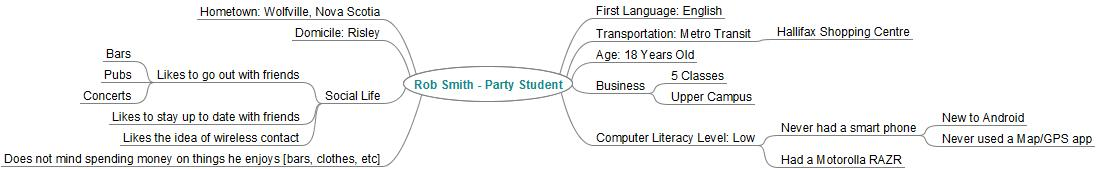
\includegraphics[width=\textwidth]{img/figure411.jpg}
        \caption{User 1: Rob Smith Brainstorm}
    \end{figure}
    \begin{figure}
        \centering
            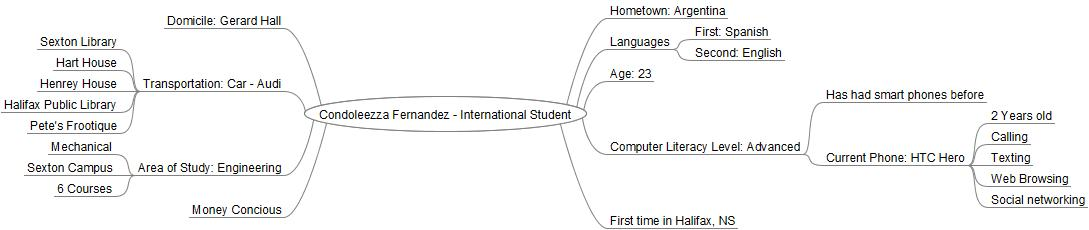
\includegraphics[width=\textwidth]{img/figure412.jpg}
        \caption{User 2: Condoleezza Fernandez Brainstorm}
    \end{figure}
    \paragraph{When looking at user personas we decided it would be best to
    create one at each end of the computer literacy and/or smartphone experience
    scale. We looked at two students; one who was born in Canada, taking Business,
    not very tech-savvy and likes to enjoy himself. The other is an international
    student who is in Mechanical Engineering, very tech-savvy, money conscious and
    on the go.}
    \paragraph{The tasks we outlined during our initial design meetings were:}
    \begin{itemize}
    \item Find/browse for a classroom on campus
    \item Find the closest wireless hotspot
    \item Find my next class with directions from current location
    \item Notify the user if they are late for a class, as well as giving directions to
    item the proper location
    \item Create a bookmark of the current location
    \item Find local restaurants
    \end{itemize}
    \paragraph{The software's architecture was broken down into two sections:
    primary functions and ideas for the software design.}
    \begin{figure}
        \centering
            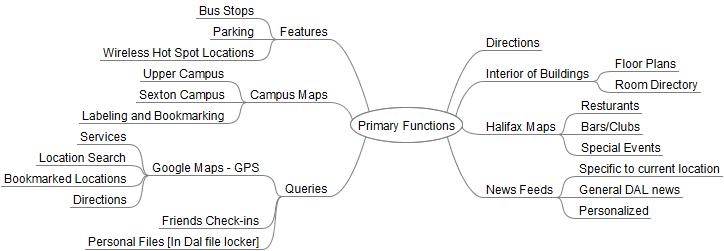
\includegraphics[width=\textwidth]{img/figure413.jpg}
        \caption{Primary Applications Functions Brainstorm}
    \end{figure}
    \begin{figure}
        \centering
            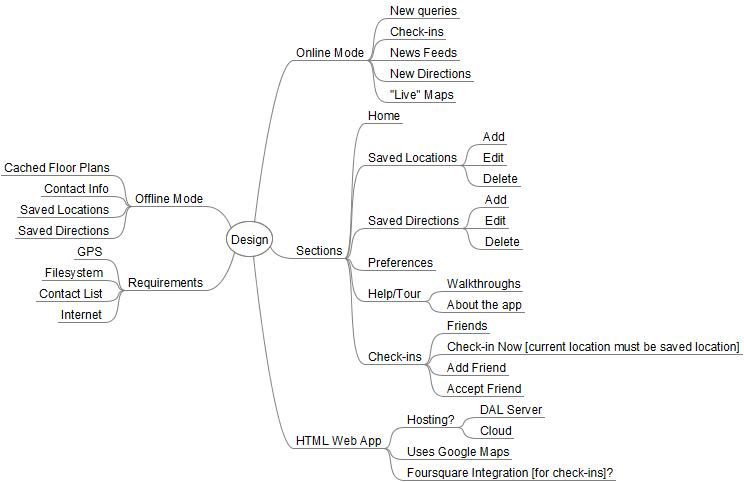
\includegraphics[width=\textwidth]{img/figure414.jpg}
        \caption{Applications Design Brainstorm}
    \end{figure}
    \paragraph{Our ideas were to either create an Android application, or an web
    application (which would allow for use on a higher number of platforms). No
    matter which platform we would choose, we planned on using Google services
    (Maps, Search, etc) to simplify the application creation. This would allow the
    application to meet the primary and secondary functionality requirements
    (showing campus buildings and services, local information, search, etc). By
    building a Dalhousie check-in feature, we give the application a social spin.}
    \paragraph{In the end we chose to program the prototype in HTML using jQuery
    Mobile as it is platform independent, easy to learn (for the less experienced
    programmers in the group), and quick to create pages.}
\section{Tasks and Users}
    \paragraph{To represent users, two personas were created with different
    backgrounds and histories of Smartphone use to provide a proper contrast for the
    testing process. Rob Smith is a 21-year-old Canadian with no history of
    Smartphone use, and would be primarily interested in the social features of the
    application. Condoleezza Fernandez is a 23-year-old mature student from
    Argentina who has a history of Smartphone use, and is primarily interested in
    the academic features of the application.}
    \paragraph{These personas were used for the first testing phase in the
    iterative process. The six use-cases (identified in the Brainstorm section) were
    divided so that each persona would "complete" three different use-cases. This
    allowed us to employ the application from a user’s perspective and get a
    firsthand look at the applications' functionality. Each of the six tasks was
    assigned a scenario that would showcase the application in a real life setting.
    For example, a potential scenario between a user and use-case would be as
    follows:}
    \paragraph{\emph{Condoleeza is studying at the Killam Library when the
    application notifies her that one of her classes begins in 15 minutes. She
    realizes that her class is just across the street and therefore has a few more
    minutes of study time. She selects the “Snooze” option which closes the
    notification. 5 minutes later the reminder pops up and notifies her that her
    class now begins in 10 minutes. Condoleezza closes the notification, packs up
    her bag, and makes it to class on time.}}
\section{Low-fidelity Prototype}
    \paragraph{When designing our prototype we decided to model the user
    interface after many popular social networking applications such as the Facebook
    or Google+ iPhone and Android applications. This means using a menu bar across
    the top--for quick navigation buttons, confirmation buttons across the bottom,
    and grids of icons for menu options within the application.}
    \paragraph{We did a first draft on paper and pencil because this allowed for
    rapid development and easy changes based on group input. The drawings were
    scanned and re-created in Adobe Flash for better clarity, coloring and easy
    transfer into the high fidelity prototype later on. Below are examples of of the
    low fidelity paper prototype and the digital low fidelity prototype:}
    \begin{figure}
        \centering
            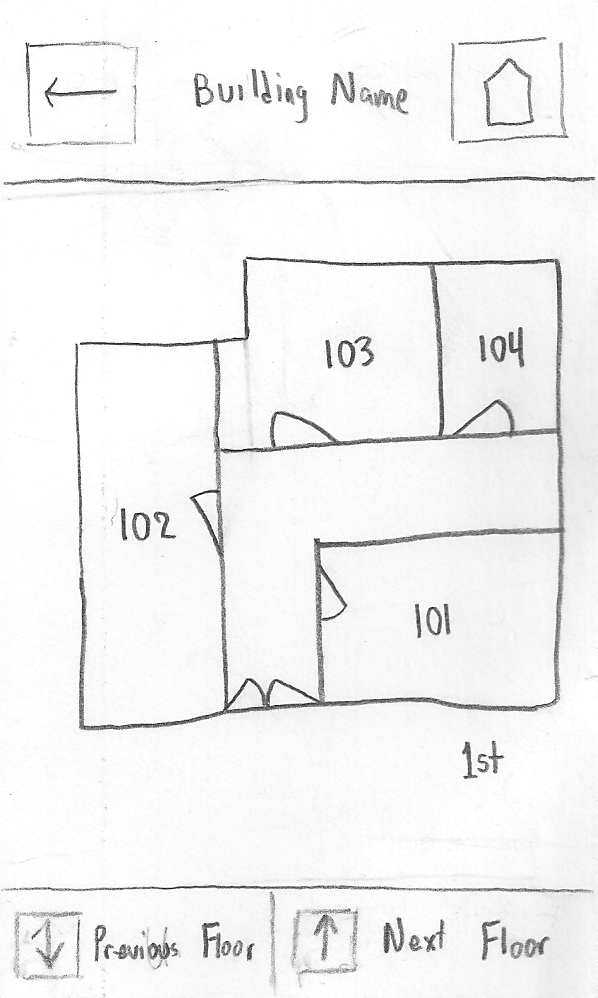
\includegraphics[height=3in]{img/figure431.png}
        \caption{Low Fidelity Hand Drawn Prototype}
        \label{fig:lfpaper}
    \end{figure}
    \begin{figure}
        \centering
            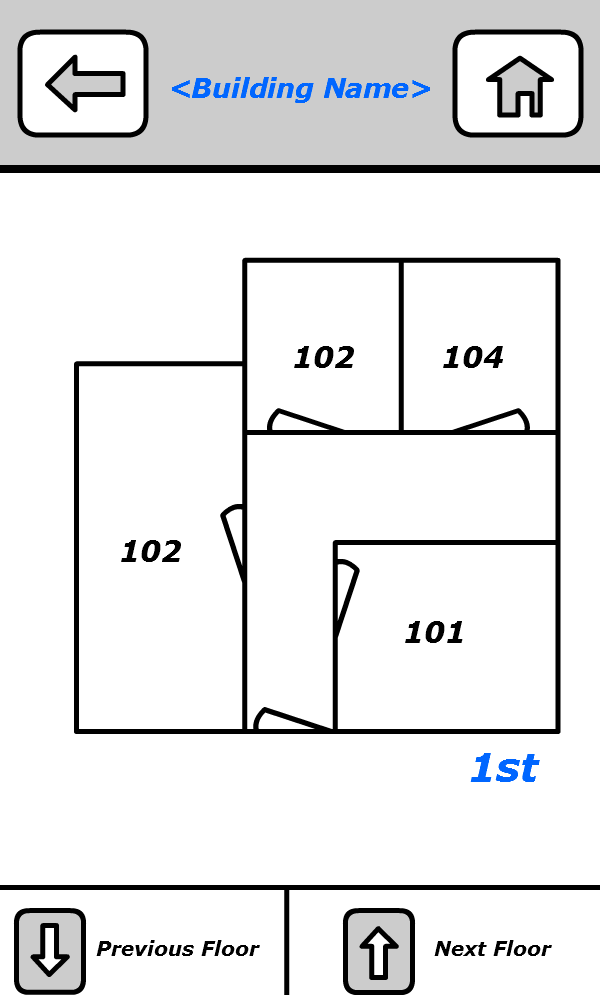
\includegraphics[height=3in]{img/figure432.png}
        \caption{Low Fidelity Digital Prototype}
        \label{fig:lfdigital}
    \end{figure}
%%%
    \paragraph{We felt that by taking design influences from Facebook and Google
    we could leverage some of the time and money they spent while designing those
    applications. Also, users of our application may be familiar with the common
    layout if they had experience with either of the previously mentioned
    applications.}
    \paragraph{We implemented a category dashboard that allowed us to group all
    of our application tasks logically so the user could move through the
    application with ease, and the interface would look aesthetically pleasing.}
    \begin{figure}
        \centering
            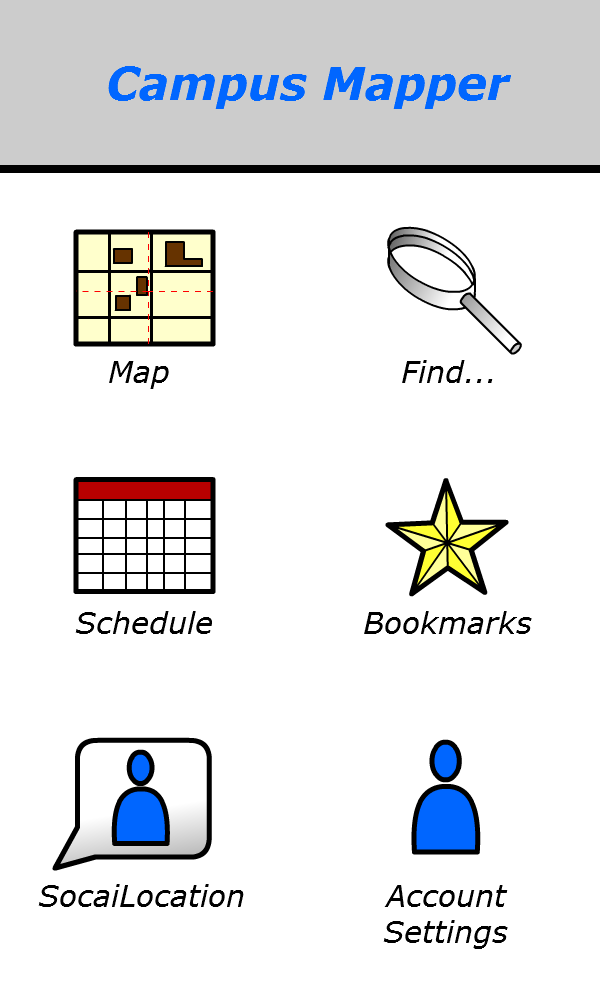
\includegraphics[height=3in]{img/figure433.png}
        \caption{The Dashboard from the Prototype}
    \end{figure}
    \paragraph{Much of what was designed at this stage was kept in the final
    prototype; as we performed user testing, most of what was changed were task
    names, slight icon changes, and the default screen that the application loads
    when it is started (straight to the map rather than the dashboard).}
\section{Cognitive Walkthrough Evaluation and Design of High Fidelity
Prototype}
    \paragraph{We next performed cognitive walkthroughs with our low fidelity
    prototype. During our walkthroughs, our testers found a few issues with our
    interface:}
    \begin{enumerate}
    \item The behaviour of the \emph{Find...} button on the main screen (Figure
    \ref{fig:digital-dashboard}) was not intuitive.
    \item The \emph{Bookmarks} label on the main page (Figure \ref{fig:digital-dashboard}) was
    confusing. The testers were not sure what type of the bookmarks the
    corresponding menu would manage.
    \item The marker icons on the \emph{Maps} page (Figure \ref{fig:digital-map}) did not clearly
    indicate that they were clickable.
    \item The \emph{Social} icon (Figure \ref{fig:digital-dashboard}`) was confusing, and did not
    clearly communicate the function of the \emph{Social} page.
    \end{enumerate}
    \begin{figure}
        \centering
            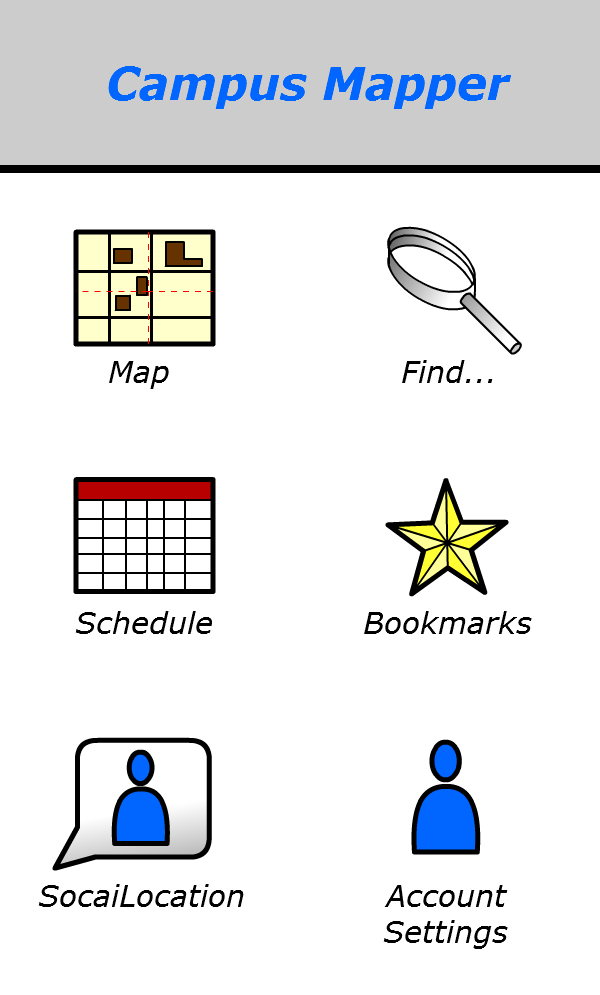
\includegraphics[height=3in]{img/dashboard.png}
        \caption{Campus Mapper Main screen, before the cognitive walkthrough changes} 
        \label{fig:digital-dashboard} 
    \end{figure}
    \begin{figure}
        \centering
            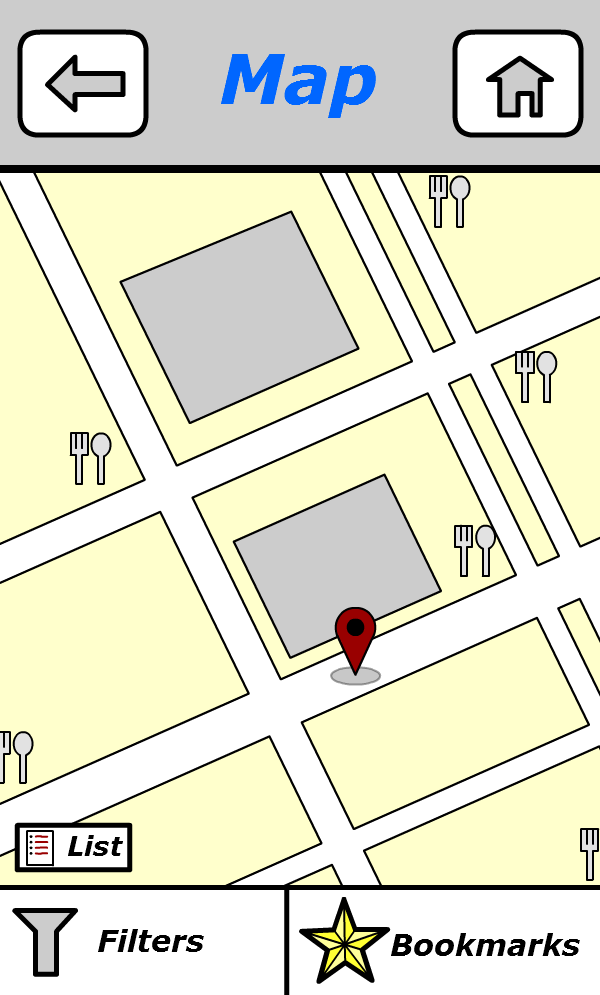
\includegraphics[height=3in]{img/map_resturants.png} 
            % Note that"resturants" is spelled wrong in the filename... 
        \caption{Campus Mapper Map screen, before the cognitive walkthrough changes}
        \label{fig:digital-map}
    \end{figure}
%%%
    \paragraph{We decided to implement the following solutions in our high
    fidelity prototype, to fix the issues that were discovered during the cognitive
    walkthroughs:}
    \begin{enumerate}
    \item We removed the Find... icon from the main page. The Find page was renamed to
    \item Find services, and can now be accessed from the Map view (Figure
    \ref{fig:cog-map}).
    \item We clarified the bookmarks issue by re-labeling the icon, as Saved locations
    (Figure \ref{fig:cog-dashboard}).
    \item We switched from floating icons to "Google thumbtack" icons (Figure
    \ref{fig:cog-map}).
    \item We changed the Social icon to a compass rose icon, as suggested by one of our
    testers (Figure \ref{fig:cog-dashboard}).
    \end{enumerate}
    \begin{figure}
        \centering
            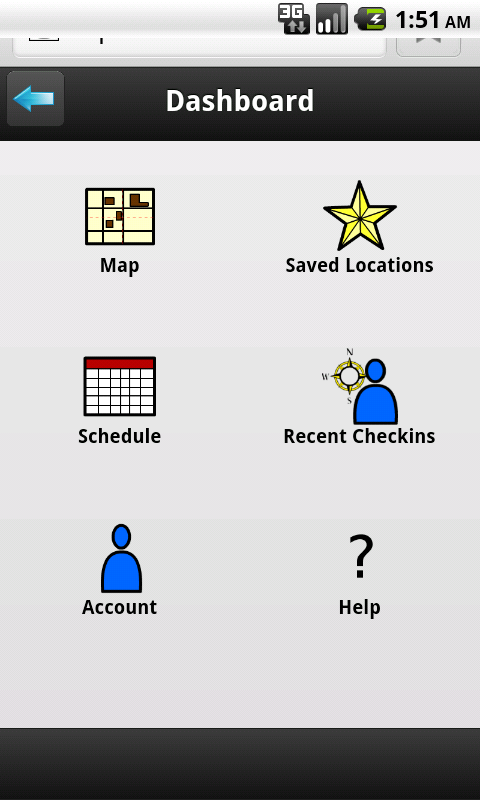
\includegraphics[height=3in]{img/cw_dashboard.png}
        \caption{Campus Mapper Main screen, after the cognitive walkthrough changes} 
        \label{fig:cog-dashboard} 
    \end{figure}
    \begin{figure}
        \centering
            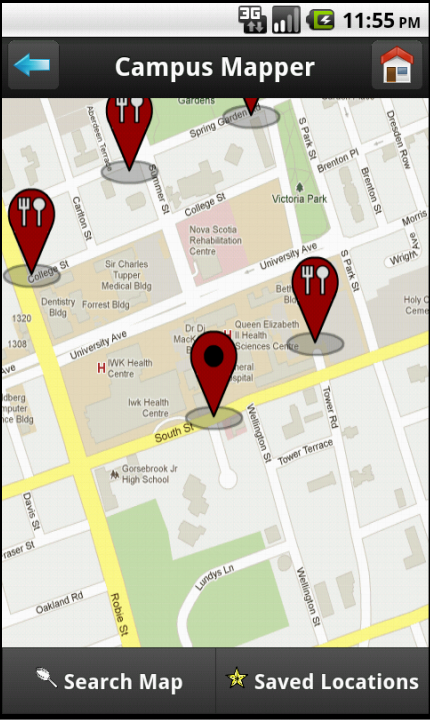
\includegraphics[height=3in]{img/cw_map-restaurant.png}
        \caption{Campus Mapper Map screen, after the cognitive walkthrough changes} 
        \label{fig:cog-map} 
    \end{figure}
    \paragraph{We made two additional changes as we implemented our high
    fidelity prototype:}
    \begin{enumerate}
    \item We re-titled the building details pages, from the specific building name to the
    static title "Details". The building name is now contained within the dynamic
    portion of each building details page.
    \item We moved the bookmark icon (a star) to the top of the building details page; it
    is now adjacent to the title.
    \end{enumerate}
\section{Heuristic Evaluation}
    \paragraph{In the last round of evaluation, several changes were made, some
    of which seem minor, but all of which led to a better overall application. The
    largest change during this stage was replacing the default screen the user would
    see, because, according to the experts in the heuristic evaluations, many people
    wanted to have the map as their first point of contact with the application.
    There were also several name changes. All of the requested and implemented
    chanies are summarized in this section, as well as the methods that were
    employed in order to generate these results.}
    \paragraph{The heuristic evaluation involved testing our high fidelity
    prototype with experts, members of our of the class, in order to see how our
    changes between the low level and high level designs improved the system, and to
    gather feedback about what else could be changed. This involved letting two
    experts separately run through the new system, make notes and fill out the
    heuristic evaluation sheets. We gave them use-cases to follow (on their
    request). We also answered experts' questions about the work flows and took
    notes on the their comments in order to gather as much information as possible.
    Finally, we discussed issues found by the experts, and, with them, developed
    solutions to improve the system.}
    \paragraph{As mentioned in the introductory paragraph of this section, one
    of the biggest features people wanted to see was the map view as the main page
    of the application. Also, there were several labeling issues that would be taken
    care of in this stage. As can be seen in figure \ref{fig:heuristic-primary}, we have moved from the
    main screen being a dashboard to it being a blank map view. We have also renamed
    "Search Map" to "Browse...", giving a clearer implication of what users should
    expect to see when they select the button. Furthermore, it was noted that the
    Search query box on the find page was not very distinguishable from the
    background; thus, it was given a clear label and a border. The difference can be
    seen in figure \ref{fig:heuristic-find}. Finally, due to experts' recommendations from the
    heuristic evaluations, school buildings have been highlighted blue in an attempt
    to make them stand out more.}
    \begin{figure}
    \centering
    \subfloat[Old Main View]{
        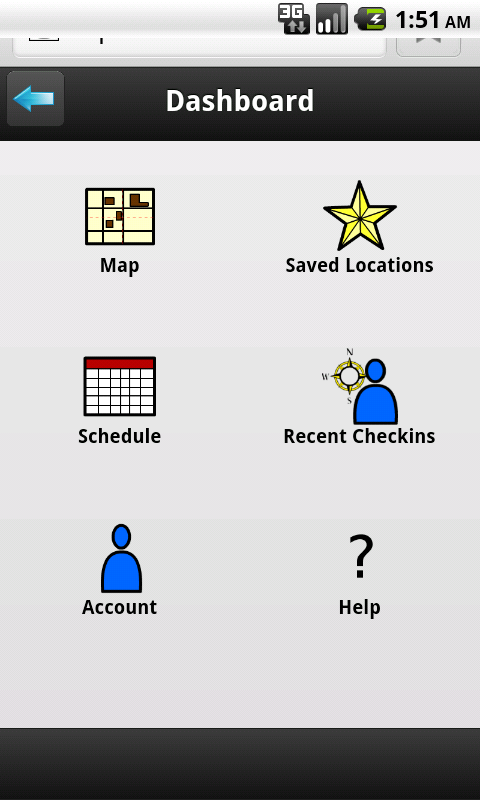
\includegraphics[height=3in]{img/pre-dashboard.png}}
    \subfloat[New Main View]{
        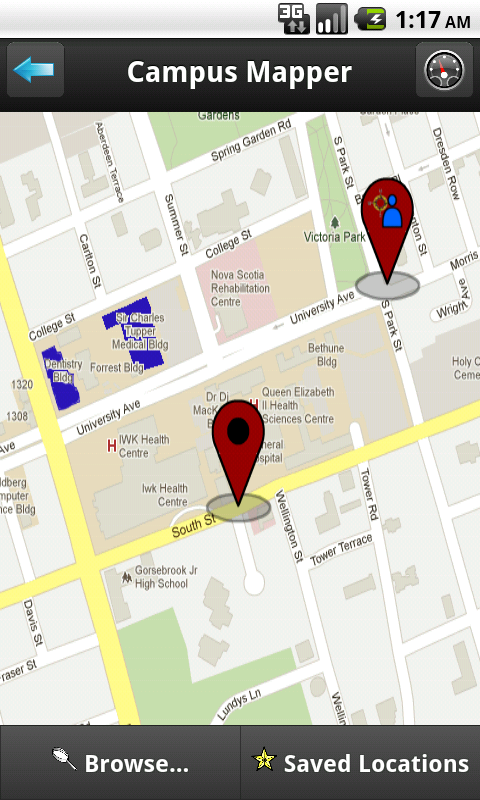
\includegraphics[height=3in]{img/post-map.png}}
    \caption{Old and new primary view}
    \label{fig:heuristic-primary}
    \end{figure}
    \begin{figure}
    \centering
    \subfloat[Old Main View]{
        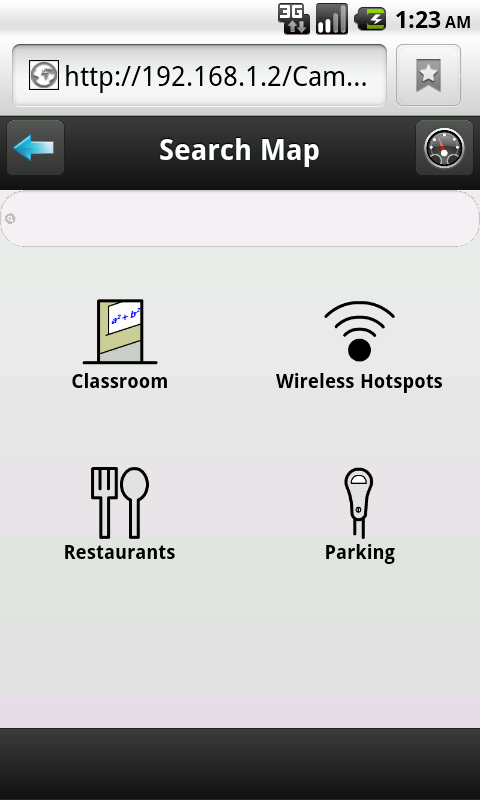
\includegraphics[height=3in]{img/pre-find.png}}
    \subfloat[New Main View]{
        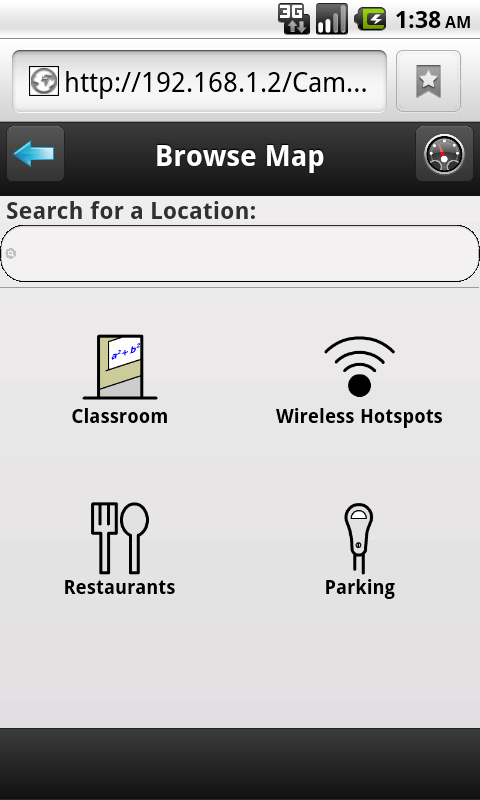
\includegraphics[height=3in]{img/post-find.png}}
    \caption{Old and new find page}
    \label{fig:heuristic-find}
    \end{figure}
%%%
    \paragraph{Further changes are also evident on the dashboard. It can be
    noted in both figure \ref{fig:heuristic-primary}
     and figure \ref{fig:heuristic-find} that the home icon has been changed
    to a dashboard icon. In addition, the help icon and saved locations icon have
    been removed from the content section of the dashboard. The help icon has been
    placed in the upper right hand corner of the dashboard, and the saved locations
    is now located solely on the map view. These changes can be seen in figure
    \ref{fig:heuristic-dashboard}. This was due to our own concerns, as we felt that it was redundant to
    have this feature in both locations, and the new placement would fit the user's
    expectations better. Another noticeable change on the dashboard regards label
    "social"; it was changed to a more appropriate title because the name "social"
    is too ambiguous, according to the experts. Thus, we believe that 'recent
    checkins' is a more explicit term of operation. Finally, the reminder dialog was
    given a line of text indicating the snooze time, as people were not aware of how
    long this would be set for. The new dialog can be seen in figure
    \ref{fig:heuristic-dialog}}
    \begin{figure}
    \centering
    \subfloat[Old Main View]{
        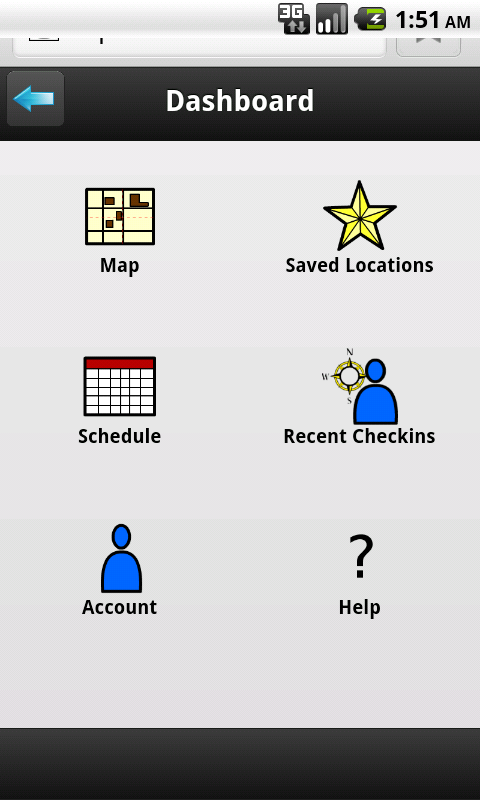
\includegraphics[height=3in]{img/pre-dashboard.png}}
    \subfloat[New Dashboard View]{
        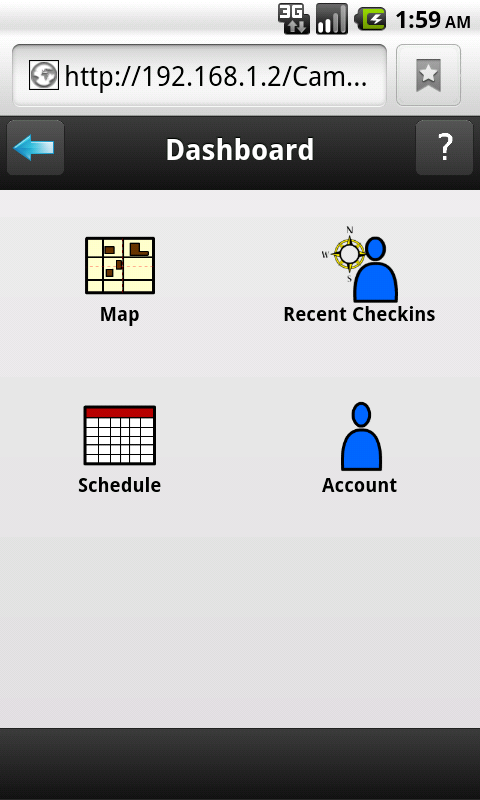
\includegraphics[height=3in]{img/post-dashboard.png}}
    \caption{Old and new dashboard.}
    \label{fig:heuristic-dashboard}
    \end{figure}
    \begin{figure}
    \centering
        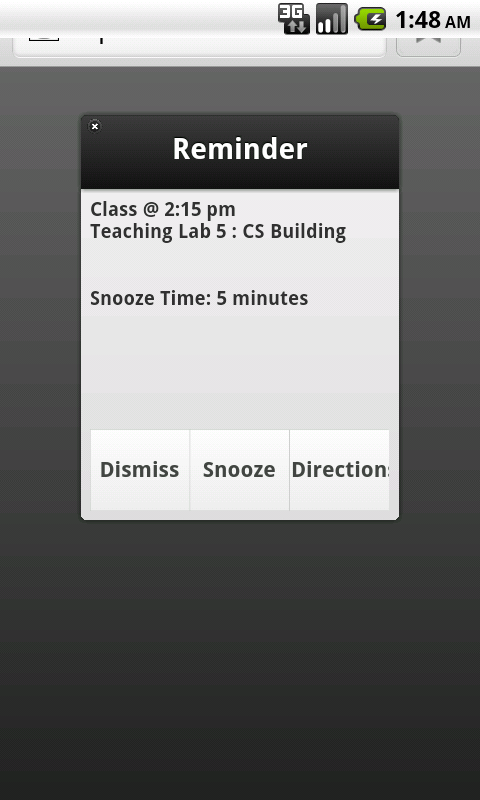
\includegraphics[height=3in]{img/post-dialog.png}
    \caption{New Reminder Dialog}
    \label{fig:heuristic-dialog}
    \end{figure}
\chapter{Conclusions and Future Work}
    \paragraph{Beginning with a simple brainstorming session, the project
    started to grow legs. We took the results of the brainstorm and put together a
    paper based prototype, modeling the interface after similar products offered by
    Google that we ourselves had used, and deemed to be ideal. The paper prototypes
    were used for cognitive walkthroughs, giving the testers a firsthand look at the
    functionality of the application. The feedback from the testing was implemented
    to make subtle changes, such as the labeling or location of certain features.
    This provided the framework for the development of the high fidelity prototype,
    which was built with jQuery Mobile and CSS.}
    \paragraph{After rounds of testing and applying valuable user feedback into
    the development of our application, we had completed the requirements for the
    application, designed an easy to use interface, and had given it the name
    ‘Campus Mapper’.}
    \paragraph{As it was previously stated, our goal for this project was to
    develop a Smartphone application that would help new students in navigating the
    Dalhousie campus. Since the primary focus was on creating a user friendly
    interface and there was insufficient time to fulfill all the system requirements
    in a single term, the program itself is not fully functional. However, if we
    were to continue working on our application, there are a few minor changes we
    would implement to make it more useful. First off, it was decided in the late
    stages of user testing that the program would ideally load the map screen on
    startup and have the user access the ‘find’ features from this screen,
    essentially combing the two most commonly used aspects into a single interface.
    We would also invest more effort into either creating or buying a set of
    application-icons that would be unique to our program.}
    \paragraph{The application we created could easily be extended into a fully
    functional website for the university where features such as finding directions
    could be printed off instead of only being viewed from a handheld device. This
    way Dalhousie students who do not own a Smartphone would still be able to take
    advantage of what our program has to offer.}
\nocite{*}
\bibliography{bib}{}
\bibliographystyle{acm}
\end{document}
